% Example template for using the unmeethesis style
% This example is for a Master's candidate in Mathematics
% It contains examples of front matter and most sections that the
% typical graduate student would need to include
% By: N. Doren 02/10/00
%     Minor mods by N. Doren 08/26/11

% Use the following specification for BOTTOM page numbering:
\documentclass[botnum, fleqn]{unmeethesis}
% OR
% Use the following specification for TOP page numbering:
% \documentclass[fleqn]{unmeethesis}
\usepackage{amsmath}
\usepackage{hyperref}
\usepackage{algorithm}
\usepackage[noend]{algpseudocode}

\makeatletter
\def\BState{\State\hskip-\ALG@thistlm}
\makeatother

\begin{document}

  \frontmatter

  % Uncomment the next command if you see weird paragraph spacing:
  % That is, if you see paragraphs float with lots of white space
  % in between them:

  % \setlength{\parskip}{0.30cm}

  \title{Distributed Video Analysis for the  Advancing  \\
  Out of School Learning in Mathematics and Engineering Project}

  \author{Cody Wilson Eilar}
  \degreesubject{M.S., Computer Engineering}
  \degree{Master of Science \\ Computer Engineering}
  \documenttype{Thesis}
  \previousdegrees{B.S., University of New Mexico, 2010}
  \date{July, \thisyear}

  \maketitle

  %\makecopyright
  %Copyright page is no longer necessary D. Murrell


  \begin{acknowledgments}
    \vspace{1.1in}
    I would like to thank my advisor, Professor Marios Pattichis, for his
    continuous support in reviewing my source code and for helping me shape my
    ideas for this thesis. I would also like to thank Elmyra Grelle for helping
    me stay on track with all the necessary requirements to graduate. Finally, I
    would like to thank Sandia National Laboratories for supporting me
    financially in my academic endeavors.
  \end{acknowledgments}

  \maketitleabstract %(required even though there's no abstract title anymore)

  \begin{abstract}
    This thesis proposes a distributed processing system for analyzing
    videos acquired through the advancing out of school learning in
    mathematics and engineering (AOLME) project. The
    proposed architecture is demonstrated by detecting writing and typing
    activities based on the Video Distributed Analysis (VIDA) system. VIDA
    leverages Amazon Web Services (AWS) to optimally distribute segments of
    video to a heterogenous compute cloud consisting of machines that have both
    CPU and GPU processing hardware onboard. The master node is responsible for
    distributing the videos and the slave nodes perform feature reduction on the
    videos by calculating a handful of cumulative distribution functions (CDF)
    to then be returned to the master node to then be classified by support vector
    machines (SVM). This thesis will demonstrate the accuracy,
    scalability and flexibility of VIDA for videos collected through AOLME. Furthermore,
    this thesis delves into the architectural details essential to distributed
    video processing on cloud infrastructures .

    \clearpage %(required for 1-page abstract)
  \end{abstract}

  \tableofcontents
  \listoffigures
  \listoftables

  \begin{glossary}{Longest  string}
    \item[$a_{lm}$]
    Taylor series coefficients, where $l,m = \{0..2\}$
  \end{glossary}

  \mainmatter

  % Include the topic chapters
  \chapter{Introduction}
There is strong interest in the development of distributed video analysis
systems that can be used to analyze large video databases. Unfortunately, the
overwhelming majority of software packages for automated video analysis, are not
necessarily designed to scale in order to handle processing on vast video
databases.

An example of a large-scale video database is  provided by the advancing out of
school learning in mathematics and engineering (AOLME) project. AOLME contains
over a thousand hours of high quality video data that need to be analyzed so as
to understand how middle school students acquire basic programming skills.
Currently, most of this analysis is done manually \cite{LopezLeiva2016} to
extract pertinent features for researchers to analyze.

Manual video annotation and transcription is extremely tedious and unsustainable
for large datasets. Because of these inhibitory factors, most of these
encoded videos are left untouched and unanalyzed, potentially leaving thousands
of hours of valuable information about the learning process unexplored and
underutilized.  Clearly there is a need for a tool to aid researchers in
properly analyzing these video datasets efficiently.

\section{\label{section:motivation}Motivation}

Current methods in video analysis systems are extremely application dependent
and are inadequate computationally to sufficiently
investigate video datasets at such a large scale. As such, there is a propensity
for a system that is accurate, scalable and flexible in nature to handle a
variety of challenges in automated video analysis.

Computationally, there is clearly a need for video analysis methods that can be
efficiently implemented in heterogenous compute hardware (such as GPUS and
CPUS), and have said hardware function in a distributed environment. Being able
to leverage heterogenous computer hardware greatly increases the efficiency and
speed of certain, heavily used, video processing algorithms such as 2D
convolutions. Furthermore, having this system exist in a distributed environment
will greatly speed up ephemeral operations and makes it possible to scale up to
address large scale problems. Thus this thesis is motivated by the challenges
associated with analyzing large scale video databases.

\section{\label{section:thesis_statement}Thesis Statement} The thesis of this
research is that it is possible to scale, accurately classify and process videos
using our proposed video analysis architecture for human activity recognition.
The basic idea is to effectively distribute the computation among compute nodes
and collect the results in the master node. The focus is to pre-compute the
computationally intensive feature extractions such as Farneback, Lucas-Kanade
optical flow and SVMs powered by a highly scalable computing architecture, and
exposing those features to researchers so that classification algorithms can  be
developed much quicker and in an interactive way. We show that large amounts of
video data can be accurately classified and that our technique is scalable.
Figure \ref{fig:typing_writing} illustrates the types of pre-cropped videos that
we are attempting to classify.

\begin{figure}[h]
  \label{fig:typing_writing}
  \centering
  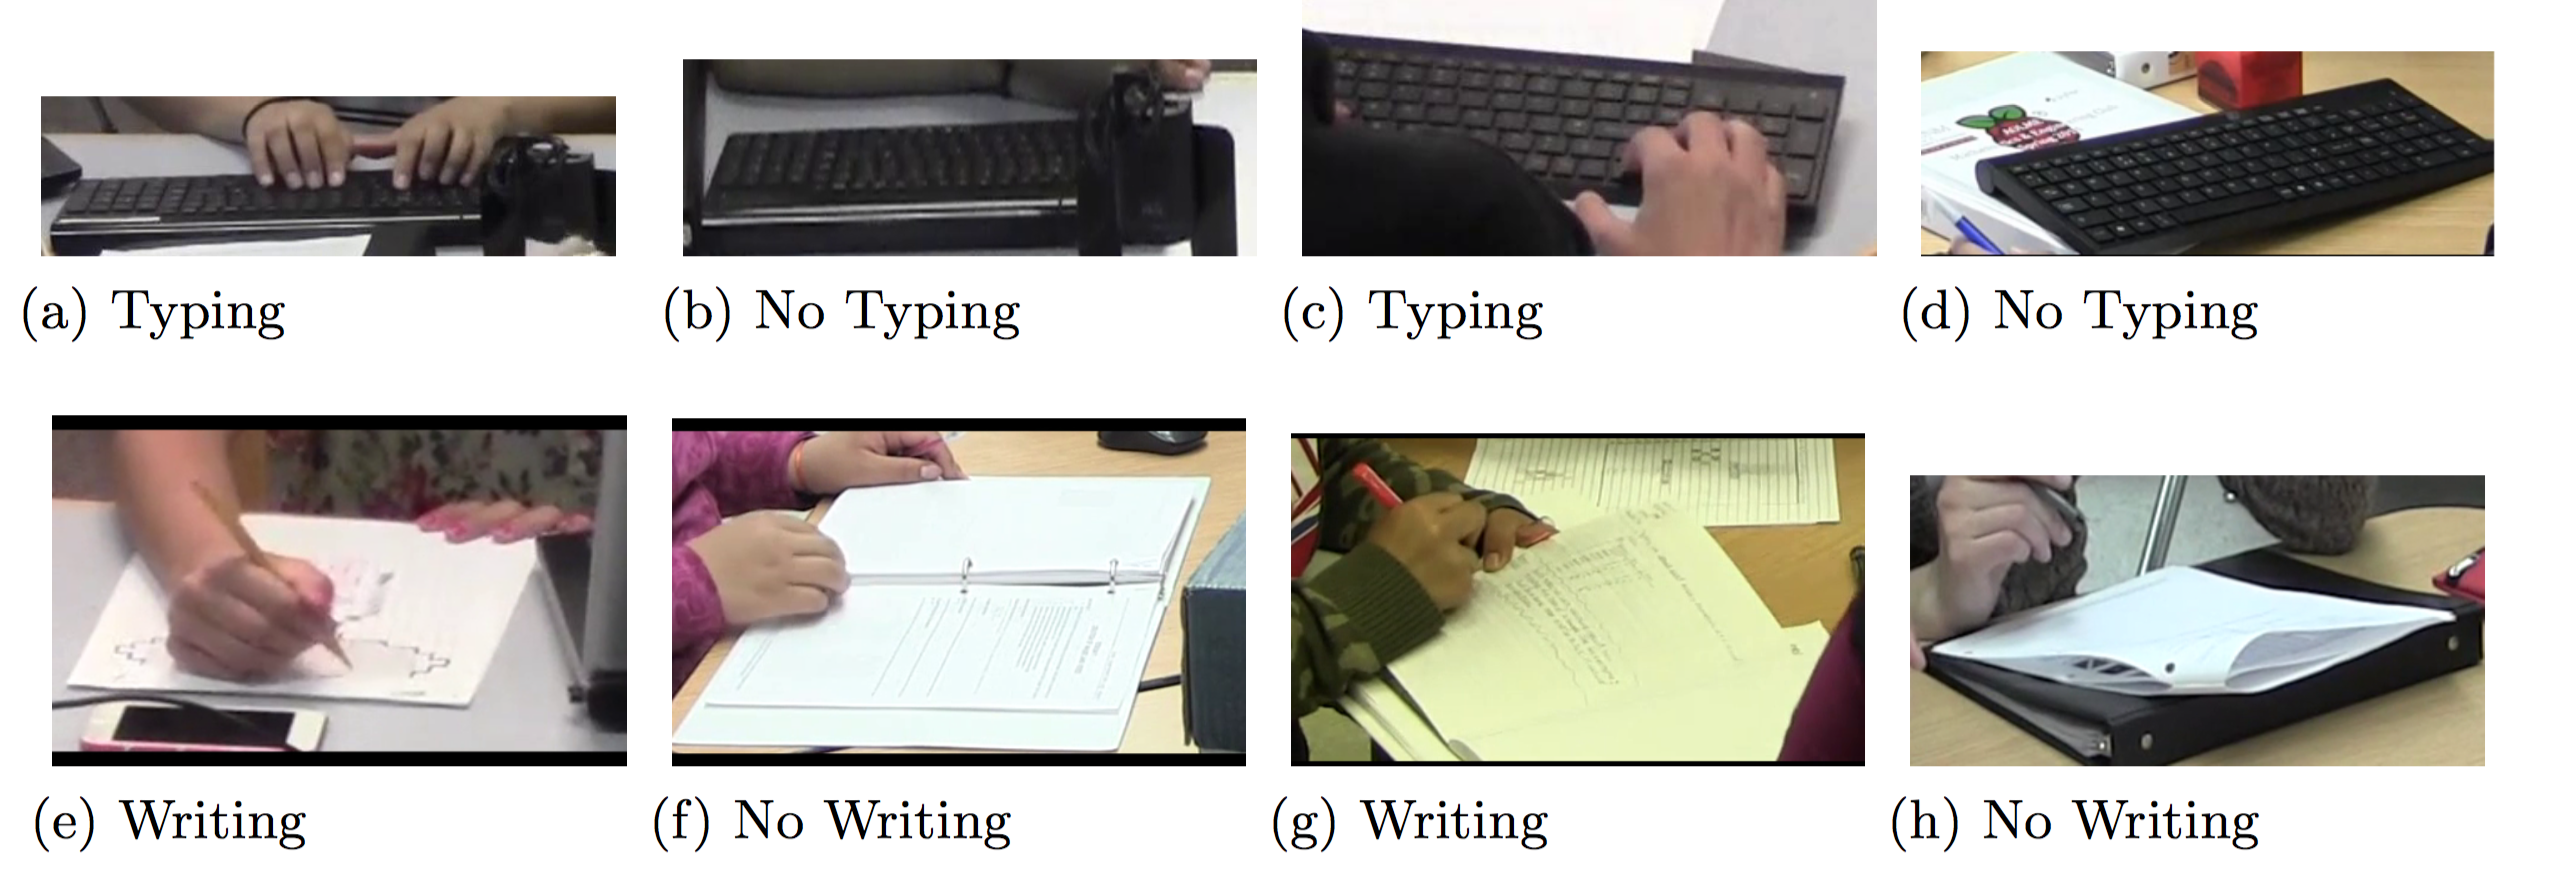
\includegraphics[width=\textwidth]{figures/typing_writing_clip}
  \caption{Example of features that have been manually extracted from the dataset
  for training and testing. For the above example, we need to classifiers for each
  activity to determine if the activity is being performed, or it is not.}
\end{figure}

\section{\label{section:contributions}Contributions}
This thesis contributes to the computer engineering community by providing both
algorithms and an architecture for efficient, scalable and rapid processing of
extremely large video datasets in a cloud environment. Additionally, all
the code written for this thesis is distributed under the MIT open source license
so that the software can be used freely in the community and will thus facilitate
reproducibility and extensibility in this field of research.

\section{\label{section:summary}Summary}
In this thesis, we show that it is possible to reduce the feature set of
videos on the order of Megabytes down to tens of Kilobytes, and then accurately
classify those features at 90\% as a particular human activity. We also create
an architecture that is capable of scaling to dozens of compute notes, and
potentially hundreds thus making the heavy lifting operations, such as computing
optical flow vectors, a trivial task that can be efficiently performed in the
AWS cloud, thus enabling researchers to extract germane features from videos in a
matter of minutes instead of hours.

  \chapter{Activity Classification in Videos}
One of the main objectives of this research is to provide a reliable method for
activity classification in videos. For this thesis, two activities of interest
to the College of Education are studied: when students are writing and when they
typing. The idea being that if we can prove that classification using ViDA works
for simple activities, we can extend the system to handle other activities just
by changing the training data and training a new classifier on that data, making
the system extremely flexible. This chapter reviews the basic techniques that
are used for reducing the feature space of videos so that any machine learning
algorithm, such as an SVM, can be used to classify the activities. It explains
the basic implementation of the Farneback optical flow algorithm
\cite{farneback2003two}, also known as dense optical flow, how the optical flow
features are further reduced, and finally the methods used to classify the
activity in the video.

\section{\label{section:optical_flow_methods}Optical Flow Methods}
In this thesis we attempt to classify two types of activities in video,  typing
and writing. Since both of these activities involve motion, i.e. a change of
apparent structure position from one video frame to the next, optical flow
algorithms  are a suitable tool for attempting to extract germane features from
the video.

Currently, there are several varieties of optical flow algorithms that have been
published. We use both Lucas-Kanade \cite{lucas1981iterative} and the Farneback
\cite{farneback2003two}  optical flow algorithms to attempt to extract
important motion features from the AOLME videos. Although as we see with our
experiments, that the Farneback algorithm is better suited for pulling out
motion features that our unique to the particular motion for which we attempt
to find in our videos. In either case, both algorithms attempt to solve
Equation \ref{eq:delta_image}

\begin{equation}
I(x,y,t) = I(x+dx, y+dy, t+dt)
\label{eq:delta_image}
\end{equation}

where $I$ is the the image, $x$ \& $y$ are the column row coordinates
respectively, and $t$ is the time between two adjacent image frames. Taking the
Talylor series expansion of Equation \ref{eq:delta_image} results in Equation
\ref{eq:taylor_expansion}


\begin{equation}
f_x u + f_y v + f_t = 0
\label{eq:taylor_expansion}
\end{equation}

where

\begin{equation}
f_x = \frac{\partial f}{\partial x} \; ; \; f_y = \frac{\partial f}{\partial y} \\
u = \frac{dx}{dt} \; ; \; v = \frac{dy}{dt}
\label{eq:taylor_expansion_partial}
\end{equation}

 Equation is \ref{eq:taylor_expansion_partial} is known as the Optical Flow
 equation. The object is determine what $u$ and $v$ are given that $f_x$ and
 $f_y$ are the image gradients and $f_t$ is the time gradient. Since in Equation
 \ref{eq:taylor_expansion} we have two unknowns, we cannot solve the system
 without additional constraints. This is known as the \textit{aperture problem}.
 Both the Lucas-Kanade method and the Farneback method attempt to estimate this
 problem. Lucas-Kande attempts to reframe the problem such that we have an
 overdetermined system, solving it and then providing motion vectors for only
 features that move. The Farneback solution, on the other hand, argues that is
 possible to solve the \textit{aperture problem} by first approximating each
 neighborhood of both frames with quadratic polynomials, and then estimating the
 displacement fields between the frames using polynomial expansion. Rather than
 providing only a few motion vectors, the Farneback method provides dense
 optical flow. That is to say that there is a motion vector for every pixel
 between the frames \cite{farneback2003two}.

\subsection{\label{subsection:lucas_kanade} Lucas-Kanade Method} For this
thesis, we leverage a common C++ library that has already implemented a
specialized version of the general Lucas-Kanade algorithm which uses pyramids to
solve the optical flow at different scales of motion
\cite{bouguet2001pyramidal}. This algorithm is provided freely in a C++ computer
vision library known as OpenCV \cite{itseez2015opencv}. Essentially, this
algorithm is much like the original paper published by Lucas and Kanade, but it
solves the issue of large motions between frames. By definition, the Lucas-Kande
method assumes that the displacement of features in the image between two frames
is small and roughly constant within a pixel neighborhood. This algorithm, then,
by definition cannot handle large motions between frames, and hence the algorithm
presented in \cite{bouguet2001pyramidal} attempts to more robustly solve
optical flow and is the algorithm that is implemented in the OpenCV \cite{itseez2015opencv}
library. In our software, we use two OpenCV library calls, \texttt{goodFeaturesToTrack}
and \texttt{calcOpticalFlowPyrLK}. The first function is used to find features
that can be easily tracked from one frame to the other using the Shi-Tomasi
algorithm \cite{shi1994good}. The next method then calculates the optical flow
between the good points using the pyramidal implementation of the Lucas-Kanade
algorithm \cite{bouguet2001pyramidal}. Algorithm \ref{alg:lk_flow} outlines the general
program flow for calculating motion vectors in ViDA.

\begin{algorithm}
\caption{Calculating Lucas-Optical Flow from Videos}
\label{alg:lk_flow}
\begin{algorithmic}[1]
\Procedure{CalculateVectors}{$frame1$, $frame2$}
  \If{\text{$track\_points\_initialized$}}
  	\State $opticalflow \gets \texttt{calcOpticalFlowPyrLK}(track\_points, frame1, frame2)$
  \Else
  	\State $track\_points \gets \texttt{goodFeaturesToTrack}(frame1)$
	\State $track\_points\_initialized \gets True$
	\State $optical\_flow \gets  \texttt{CalculateVectors}(frame1, frame2)$
  \EndIf
  \Return $optical\_flow$
\EndProcedure
\end{algorithmic}
\end{algorithm}

\subsection{\label{subsection:farneback_method} Farneback Method}
Again, we leverage the C++ OpenCV library to calculate the motion vectors for
Farneback optical flow. Unlike the previous method, the Farneback algorithm does not require
any track points to estimate motion vectors because it is a dense optical flow
algorithm, i.e. 100\% of the pixels has an associated optical flow vector. The
main idea behind calculating the motion vectors in this method, is to use
polynomial expansion for a neighborhood of pixels \cite{farneback2003two} and
then use that estimation to find a global translation between the two frames. This
essentially aids with global background movement. The main algorithm used in ViDA
is similar to Algorithm \ref{alg:lk_flow} but contains fewer steps since there
is no need to get good features to track. The Farneback implementation is shown
in Algorithm \ref{alg:farneback}.

\begin{algorithm}
\caption{Calculating Farneback Flow from Videos}
\label{alg:farneback}
\begin{algorithmic}[1]
\Procedure{CalculateVectors}{$frame1$, $frame2$}
  \State $optical\_flow \gets \texttt{calcOpticalFlowFarneback}(frame1, frame2)$\\
  \Return $optical\_flow$
\EndProcedure
\end{algorithmic}
\end{algorithm}

\subsection{\label{subsection:comparison}Comparison of Methods}
We implemented the Lucas-Kanade method first in our research because in general,
performance is a concern and, as long as not too many features or
too few features are detected, the Lucas-Kanade algorithm will be faster
\cite{de2015choosing}. Despite this fact, we found that our classifier did
not perform as well on features extracted from the Lucas-Kanade method, as it
did using the Farneback method. As a result, most of the results in this thesis
have been calculated with Farneback optical flow unless otherwise specified.

\section{\label{section:feature_extraction}Feature Extraction from Optical Flow}
The \texttt{CalculateVectors} function in both Algorithm \ref{alg:lk_flow} and
\ref{alg:farneback} returns several dense matrices that represent the features
that we can extract from the optical flow output. These features are magnitude,
orientation, x direction and y direction of the optical flow features. These
are ultimately the features that we use to train and classify using an SVM. However,
if we had two $N \times M$ video frames as the input, we now have $4 \times N \times M$
features. Clearly we have not yet reduced the input feature space. Thus, based
on information that we know \textit{a-priori}, we can reduce our feature space
significantly.

In the case of typing and writing, we know we can expect there to be motion from
one frame to the next. We don't know by how much, but we do know that it is not
zero. Using this knowledge, we can then threshold the optical flow vectors that
we get back from Algorithms \ref{alg:lk_flow} and \ref{alg:farneback}. The
threshold value used was empirically calculated from doing multiple runs on the
AOLME videos. We found we got the best results by only retrieving
optical flow vectors with a magnitude greater than 75\% of the max value. The set
of Equations in \ref{eq:optical_threshold} illustrate this idea.

\begin{align}
  \label{eq:optical_threshold}
  \begin{split}
  \mathbf{V} &= (\mathbf{V_x}, \mathbf{V_y}) \\
  \mathbf{V_m} &=
  \begin{cases}
    1, & \text{if } \|\mathbf{V}\| \geq \max( \|\mathbf{V}\|) \times 0.25 \\
    0, & \text{otherwise}
  \end{cases}
  \end{split}
\end{align}

where $\mathbf{V_x}$ and $\mathbf{V_y}$ are the optical flow vectors in the
x and y directions respectively. $\mathbf{V_m}$ is the bit mask that is
then used to extract the subset of data from each of the dense matrices.

\begin{align}
  \label{eq:subset}
  \begin{split}
  \text{Let: } \\
  \|\mathbf{V\prime}\| &= \|\mathbf{V}\| \circ \mathbf{V_m}\\
  \mathbf{V_x\prime} &= \mathbf{V_x} \circ \mathbf{V_m}\\
  \mathbf{V_y\prime} &= \mathbf{V_y} \circ \mathbf{V_m}\\
  \mathbf{\Phi\prime} &= \mathbf{\Phi} \circ \mathbf{V_m}
\end{split}
\end{align}

Using the optical flow bitmask, $\mathbf{V_m}$, we can then extract features
from each one of our dense matrices using the Hadamard product as shown in
Equation \ref{eq:subset}, where $\|\mathbf{V\prime}\|,
\mathbf{V_x\prime},\mathbf{V_y\prime}, \mathbf{\Phi\prime}$ are subset matrices
for the magnitude, x and y direction and orientation respectively. We have now
reduced the feature space somewhat, but depending the size of the video and the
amount of entropy per frame pair, we could still have a significant amount of
data to process for classification.

In addition to extracting generic vectors from the video, we also add
geometrical centroids, blob orientation and background motion around the blobs
to the optical flow statistics being used for classification. We implement these
methods to attempt to leverage information that could be useful during
classification. In order to calculate the geometrical centroids and orientations
of each blob, we use some well known algorithms available in OpenCV,
\texttt{connectedComponentsWithStats} and \texttt{findContours}
\cite{itseez2015opencv}. \texttt{connectedComponentsWithStats} is a function
that allows us to compute the centroid for each blob of connected pixels. The
input to this function is our binary mask image, $\mathbf{V_m}$. Once we have
all the connected blobs, we can then calculate the orientation of each one of
those blobs using \texttt{findContours} in combination with with
\texttt{fitEllipse}. The full implementation of this algorithm is outlined in
Appendix \ref{ap:centroids}. The final step is to then dilate each blob, and
then calculate the optical flow statistics in the difference region. Figure %todo
and Figure blah illustrate the concept of the above steps. 

\section{\label{section:classification}Classifying the Reduced Feature Space}

  \chapter{Architecture of Video Distributed Analysis}
\section{\label{section:cloud_computing}Cloud Computing with Amazon Web Services}


  \chapter*{Appendices}

  \addcontentsline{toc}{chapter}{Appendices}
  % Next lines duplicated from .toc file and used to create mini
  % "Appendix Table of Contents," if desired:
  %\contentsline {chapter}{\numberline {A}Proving $E=MC^2$}{4}
 % \contentsline {chapter}{\numberline {B}Derivation of $A = \pi r^2$}{5}
  % End mini table of contents

  \appendix
  \chapter{Proving $E=MC^2$}
  I refer the reader to many of grandpa's famous books on this subject.
  \chapter{Derivation of $A = \pi r^2$}
  A circle is really a square without corners.  QED.

  \bibliographystyle{acm}
  \bibliography{ivpcl_publications}

\end{document}
